\documentclass[10pt, a4paper, twosize]{article}
%\documentclass[12pt, a4paper, twoside]{book}

\usepackage{helvet}
\usepackage{hyperref}
\usepackage{graphicx}
\usepackage{listings}
\usepackage{textcomp}
\usepackage[
	a4paper,
	outer=2cm,
	inner=4cm,
	top=2cm,
	bottom=2cm
]{geometry}
\usepackage{float}
\usepackage{tabularx}
\usepackage[disable]{todonotes}
\usepackage{color, soul}
\usepackage{amsmath}
\usepackage{algorithmicx}
\usepackage[noend]{algpseudocode}
\usepackage{algorithm}
\usepackage{framed}
\usepackage{subcaption}
\usepackage{titlepic}
\usepackage{fancyhdr}
\usepackage[simplified]{styles/pgf-umlcd}
\usepackage{shorttoc}
\usepackage{url}
\usepackage{paralist}

\definecolor{grey}{rgb}{0.9, 0.9, 0.9}
\definecolor{dkgreen}{rgb}{0,0.6,0}
\definecolor{dkred}{rgb}{0.6,0,0.0}

\lstdefinestyle{DOS}
{
    backgroundcolor=\color{black},
    basicstyle=\scriptsize\color{white}\ttfamily,
    stringstyle=\color{white},
    keywords={}
}

\lstdefinestyle{makefile}
{
    numberblanklines=false,
    language=make,
    tabsize=4,
    keywordstyle=\color{red},
    identifierstyle= %plain identifiers for make
}

\lstset{
  language=Java,                % the language of the code
  basicstyle=\footnotesize\ttfamily,
  numbers=left,                   % where to put the line-numbers
  stepnumber=1,                   % the step between two line-numbers. If it's 1, each line
  numbersep=5pt,                  % how far the line-numbers are from the code
  backgroundcolor=\color{white},      % choose the background color. You must add \usepackage{color}
  showspaces=false,               % show spaces adding particular underscores
  showstringspaces=false,         % underline spaces within strings
  showtabs=false,                 % show tabs within strings adding particular underscores
  frame=single,                   % adds a frame around the code
  rulecolor=\color{black},        % if not set, the frame-color may be changed on line-breaks within not-black text (e.g. comments (green here))
  tabsize=2,                      % sets default tabsize to 2 spaces
  captionpos=b,                   % sets the caption-position to bottom
  breaklines=true,                % sets automatic line breaking
  breakatwhitespace=false,        % sets if automatic breaks should only happen at whitespace
  keywordstyle=\color{blue},          % keyword style
  commentstyle=\color{dkgreen},       % comment style
  stringstyle=\color{dkred},         % string literal style
  columns=fixed,
  extendedchars=true,
  frame=single,
}

%\renewcommand{\chaptername}{Topic}

% New definitions
\algnewcommand\algorithmicswitch{\textbf{switch}}
\algnewcommand\algorithmiccase{\textbf{case}}
\algnewcommand\algorithmicassert{\texttt{assert}}
\algnewcommand\Assert[1]{\State \algorithmicassert(#1)}%
% New "environments"
\algdef{SE}[SWITCH]{Switch}{EndSwitch}[1]{\algorithmicswitch\ #1\ \algorithmicdo}{\algorithmicend\ \algorithmicswitch}%
\algdef{SE}[CASE]{Case}{EndCase}[1]{\algorithmiccase\ #1}{\algorithmicend\ \algorithmiccase}%
\algtext*{EndSwitch}%
\algtext*{EndCase}%

\pagestyle{fancy}
\fancyhf{}
\fancyhead[RO, LE]{\small \rightmark}
\fancyfoot[RO, LE]{\small \thepage}

\begin{document}

%\frontmatter

\begin{titlepage}
\vspace*{5cm}
\begin{center}

\includegraphics[width=.5\textwidth]{images/EdNapUniLogoCMYK}~\\[1cm]

\textsc{\Large Edinburgh Napier University}\\[1.5cm]

\textsc{\LARGE \bfseries SET08101 Web Tech}\\[0.5cm]

\hrulefill \\[0.4cm]
{\huge \bfseries Lab 5 - More JS \& Some Design \\[0.4cm] }
\hrulefill \\[1.5cm]

\begin{minipage}{0.4\textwidth}
\begin{flushleft} \large
\textbf{Dr Simon Wells} \\
\end{flushleft}
\end{minipage}

\vfill

\end{center}
\end{titlepage}

%\shorttoc{Overview}{0}

%\setcounter{tocdepth}{2}
%\cleardoublepage
%\tableofcontents
%\listoffigures
%\listofalgorithms
%\addtocontents{toc}{~\hfill\textbf{Page}\par}

%\mainmatter

%\input{sections/labs/04_ui}

\section{Aims}
\paragraph{} At the end of the practical portion of this topic you will:

\begin{itemize}
\item Have practised you JavaScript to solve an actual programming problem.
\item Integrated some HTML, CSS, \& JS to create an entire single page site that solves a problem.
\item Have some idea of the range of tools and techniques available for prototyping both web pages and the network of relationships between pages in a site that you're designing.
\item Used placeholder text generation tools to help you lay out portions of pages before the final content is ready.
\item Used colour tools to select a palette of visually appealing and accessible colours for use on a site.
\item Investigated and applied style guides to the design of a website.
\end{itemize}

\begin{framed}
{\bf{NOTICE:}  Some of the exercises today build upon learning from previous weeks. Importantly, you should be noticing that many of the techniques and concepts we have studied so far will draw together to help you tackle the first coursework assignment.}
\end{framed}


\paragraph{} Many coders say that they ``can't do design'' but that is untrue. You don't need to be a graphic designer in order to produce solid, pleasing, and usable designs. All you really have to do is practise a few tools that give short-cuts to some of the more difficult tasks like selecting colours and to follow some simple design principles, like keeping things simple and uncluttered, rather than crowded. Do this, practise, and maintain a critical eye for your own and other's designs and you will soon be able to produce acceptable website designs. Remember, your site does not have to be the most beautiful, artistic, or novel in the world, it just has to communicate your data to your user. This is it's primary job. So you should be considering order of data, arrangement of data, linking between and within data, how data can be broken into various subsections or pages. This will all inform the design of your overall navigation and how your individual pages should be laid out. 

\section{Activities}

\paragraph{} First we'll do a short programming exercise that intergrates HTML, CSS, and JS. Then we'll look at some design aspects.

\subsection{A ROT13 Encoder/Decoder Page}
\paragraph{} The purpose of this activity is to develop a page that will enable you to type in a message and press an ``encode'' button. Your message will then be processed using a JS version of the ROT13 algorithm. The processed or ``enciphered'' message will then be diplayed in an output area of the screen. 

\paragraph{} Our page's interface should look something similar to this:

\begin{figure}[H]
\centering
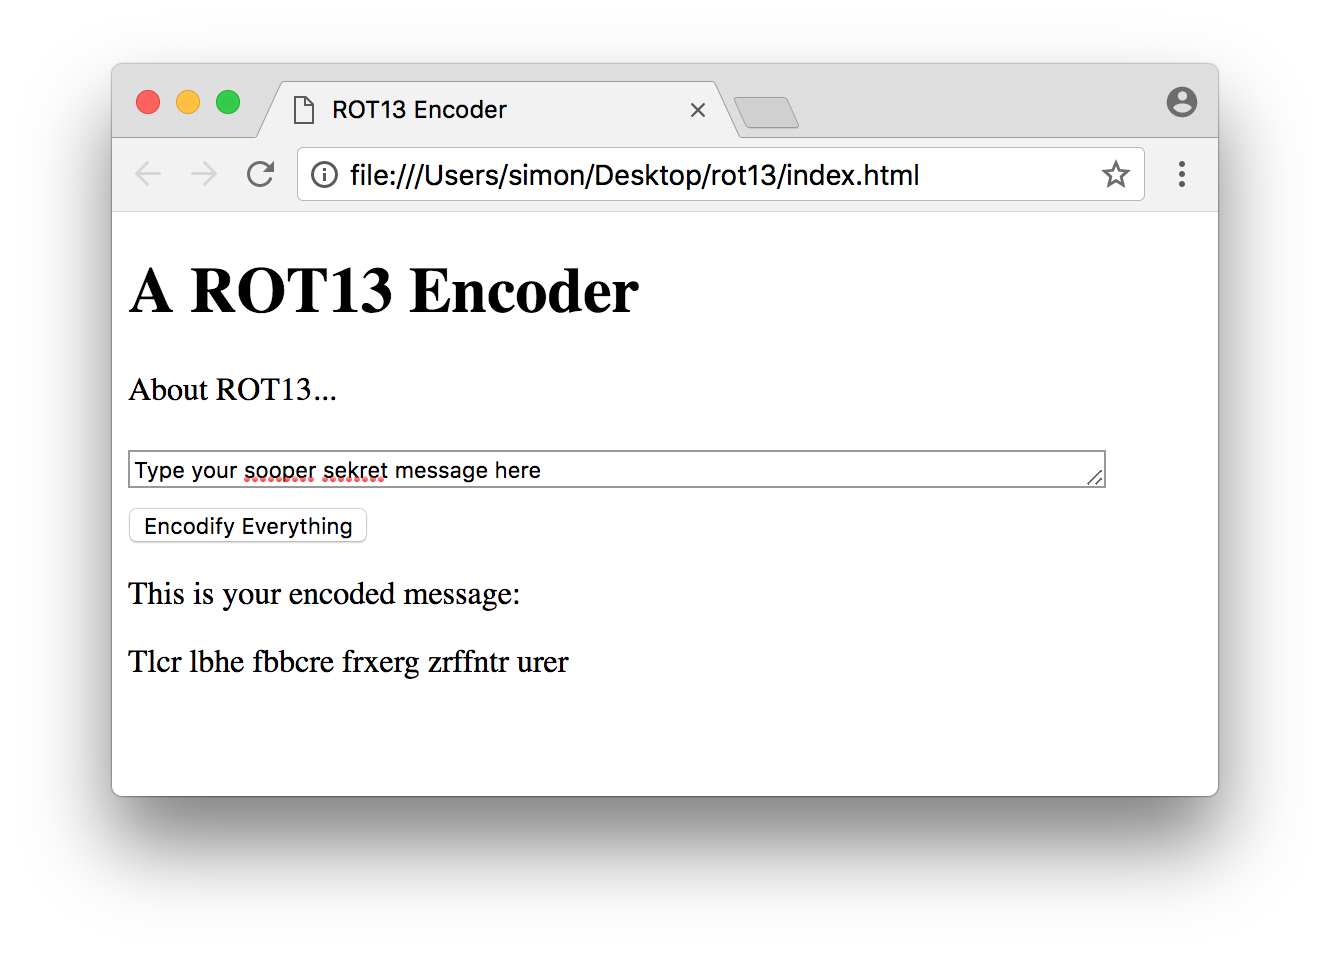
\includegraphics[width=0.85\textwidth]{images/rot13_ui}
\caption{The user interface for the ROT13 page.}
\label{fig:rot13_ui}
\end{figure}

\paragraph{} Notice that we have a few HTML interface elements on display here. We have the usual stuff, a title, heading 1, and a paragraph. We then have a textarea and a button, then what looks like a second and a third paragraph to finish the lower part of the page. I have used placeholder text for some things, especially the line starting ``About ROT13...'' -- feel free to add more text describing the ROT13 encoding process. To understand ROT13 you will have to read about it a bit so do some research and write a short paragraph describing how it works. You are more likely to actually understand something that you can explain, and you are more likely to be able to implement something that you understand.

\paragraph{} The idea is that our user types a message into the text area then presses the button. The button causes a JavaScript function to run which takes the message from the text area, encodes it using the ROT13 scheme, then displays the encoded message on the screen.

\paragraph{} Have a go at building the interface yourself\footnote{but read ahead or do some additional research if you get stuck}. What parts might you need to get this working? What files will you need to create?

\paragraph{} At the very least we will probably need an HTML file to hold the parts of the interface and display them in the browser, a CSS file to style and present the interface in the browser, and a JavaScript file to do the magic processing when the button is pressed. I have named these three files as follows:

\begin{enumerate}
\item index.html
\item rot13.css
\item rot13.js
\end{enumerate}

\paragraph{} Add enough HTML to index.html to get your CSS \& JS files linked in and so that the basic user interface elements shown above are displayed. Remember that at any point you can use a quick call to console.log() to output things to the browser's developer tools if you want to check the value of something or, for example, to check whether the button press is actually calling the JavaScript function.

\paragraph{} You should end up with something like this\footnote{Obviously you have done your own version so things might be named or arranged differently, but this should give you inspiration}:

\begin{lstlisting}
<html>
    <head>
        <link rel="stylesheet" type="text/css" href="rot13.css">
        <title>ROT13 Encoder</title>
    </head>
    <body>
        <h1>A ROT13 Encoder</h1>
        <p>About ROT13...</p>
   
        <div id="input_area">
            <textarea rows="1" cols="50" autofocus id="message">Type your sooper sekret message here</textarea>
             <button type="button" onclick="encode()" id="encode_button">Encodify Everything</button> 
        </div>
        
        <div id="output_area">
            <p>
            This is your encoded message:<br />
            <div id="output"></div>
            </p>
        <div>
        <script type="text/javascript" src="rot13.js"></script>    
    </body>
</htmL>
\end{lstlisting}

\paragraph{} Notice that we've given many HTML elements an ID so that we can access them individually from our JavaScript.

\paragraph{} I have done \emph{minimal} styling of the HTML, mostly just to make the text area a little prettier and give it some better spacing and presentation:

\begin{lstlisting}
textarea{
    border:1px solid #999999;
    width:90%;
    margin:5px 0;
}
\end{lstlisting}

\paragraph{} You can obviously style things much more copiously. Our example so far is very plain and basic HTML but feel free to enhance the presentation to your heart's content.

\paragraph{} We need to have an encode function in the rot13.js file. This function will be called every time the button is pressed in the UI. Our function outline is as follows: 

\begin{lstlisting}
function encode() 
{ 
}
\end{lstlisting}

\paragraph{} Obviously this does nothing at the moment. We will need to add code to do the following:


\begin{enumerate}
\item Retrieve the text from the text area, then,
\item For each letter in the text, find the corresponding letter that is 13 letters further along the alphabet than our input. For example, if the input is `a' then the encoded letter is `m' and if the input is `b' then the encoded letter is `n' and so on. When we get to the end of the alphabet we loop around to a again so `l' encodes for 'z' and `m' encodes for `a'.\footnote{Notice how `a' encodes for `m' and `m' encodes for `a', perhaps that will make it easy to decrypt our secret message?},
\item Store the encoded version of each letter temporarily until the message is entirely encoded,
\item Update the user interface with our encoded message.
\end{enumerate}

\paragraph{} There are some additional points to consider, what about upper and lower case? what about punctuation? I have ignored these aspects and passed the unencoded uppercase characters and punctuation straight through to the output but you might choose a different strategy such as altering the entire message to uppercase before encoding (which is a traditional solution with classical codes \& cyphers) or else handling both upper and lower case independently. From a security perspective, passing anything through from the plain text to the cypher text is a huge risk.

\paragraph{} Attempt to write the JavaScript for the encode() function using the outline above and your knowledge from your background reading. If you get really stuck there is a sample solution in Section \ref{solution}. Completing this exercise will put you in a really good position to tackle the first coursework assignment and you will find that there are many elements of the solution that can be transferred across and built upon.

\subsection{Design: Prototyping with Wireframe \& Mockup Tools}
\paragraph{} There are two key activities in the early design phase for a website. Firstly, determining what pages are required for your site and how to navigate consistently between them, and secondly, determing how the content on your pages should be arranged and laid out. Neither task can be successfully completed in isolation from the other as navigation between pages can effect navigation elements of individual pages, and the amount of content shown on a given page can affect the number or range of pages required overall for the site.

\paragraph{} There are many tools that can be used to mockup a website during the design phase. The simplest is pen \& paper, used to draw out sketches of how a page should look; where the major elements of the page should be placed in relation to each ther. Similarly, a simple diagram showing how a site can be navigated is a useful design artefact that can be produced on paper. A whiteboard and a copious supply of post-it notes is also a useful \emph{analogue} toolset as you can easily make changes to your design and move things around.

\paragraph{} It is a good idea to start sketching out a navigation tree early in the design phase, even if it just means that you have some arrows, representing hyperlinks, between boxes, representing pages. Give thoses boxes a name. You know that there will be one called index.html and perhaps others such as an about page, a help page, a contact page. You should also consider the way that your content is organised, perhaps there is a hierarchy in which your pages can be grouped and then navigated, for example, a bookshop website might have a page for each book, however, in order to navigate perhaps thousands of pages for individual books, they may in turn be organised by genre, rating, price, edition, or any number of other factors. These kinds of groupings give us a way to sort a potentially huge number of pages into a more organised and managable set of groups of pages.


\paragraph{} Almost any graphics package will support you in drawing a navigation tree. However, there are also a heap of online tools that provide methods for mocking up website designs. These are some free ones:

\begin{itemize}
\item \url{https://wireframe.cc/}
\item \url{http://mockflow.com}
\item \url{https://www.invisionapp.com/}
\item \url{https://mockingbot.com/}
\end{itemize}

\paragraph{} There are many others, a search for something along the lines of ``web design wireframe tool'' (try replacing `wireframe' with `mockup') will reveal many more . You should experiment with a few and decide if the online mockup tool is something that you want to work with. Many professional developers are happy to work with paper or whiteboard, and more generic graphcis tools so you should make a decision that works for you. One thing to now is that mockups  \& wireframes are merely prototypes. There is a range of prototypes from the lowest fidelity hand-drawn sketch right through to something built with HTML \& CSS that is just lacking content and sign-off by a decision maker. Choosing the right level of fidelity at which to prototope depends upon the time available, the complexity of the problem, and the context in which the design work is being performed, for example, if you were trying to win a contract then a medium fidelity prototype might sell your vision to a client better than a wireframe outline. You will build experience and knowledge about how best to approach the prototyping phase.

\paragraph{} Try out a few mockup tools (as well as pencil \& paper) and use them to mockup your ROT13 encoder. Try out a few alternative designs for how you would lay out your page. Consider other pages that you might have if you were to add encoders for other Cyphers, for example the Caesar Cypher\footnote{\url{https://en.wikipedia.org/wiki/Caesar_cipher}}. If you had multiple codes and cyphers then perhaps you would want an index apge that allowed you to navigate to each. Perhaps you would also have ancillary pages such as about or contact pages, Add these to your navigation tree and mockup how they would look. Think carefully about which featuers each page might need and how to present them. 


\subsection{Design: Mocking up Content with Placeholder Text}
\paragraph{} Until the actual copy for your site is written, a job that is often performed by another member of your team, or even someone outside your team entirely, it can be useful to mockup the content so that you have something to place on screen. This is particularly important as you start to move from early design toward implementation. Whilst you can just copy \& paste text from elsewhere or even just place graphical blocks to indicate where content should go, there are both some advantages and disadvantage. For example, copying \& pasting existing text from elsewhere can lead to your placeholder text becoming accidentally mixed with live content but there is the advantage of existing text at least having similar rhythms and cadences to your live text. Graphical blocks will ``block out'' where text should go but this will not have very many similarities with actual text. A solution it to use ``Greeked'' text. Text sections, usually in Latin, that have similar patterns in terms of word length and paragraph length to lots of modern languages but are difficult to mistake for those same languages. Greeking has been used for centuries as a method to get placeholder text to help lay out the printed page before the final text was ready. Whilst we aren't dealing with printed pages necessarily, there are sufficient similarities for this to be a useful technique\footnote{Not everyone agrees that Greeking is either good or useful. Some people think that the design should be done with the actual text that will be displayed on screen. Whilst this is true in an ideal world, there are many reasons which such an approach might be less pragmatic. Can you think of any reasons why you might not be able to use the actual text?}.

\paragraph{} The easiest way to take advantage of Greeking is to have a section of writing by Cicero ready to use, e.g. 

\begin{framed}
Lorem ipsum dolor sit amet, consectetur adipiscing elit, sed do eiusmod tempor incididunt ut labore et dolore magna aliqua. Ut enim ad minim veniam, quis nostrud exercitation ullamco laboris nisi ut aliquip ex ea commodo consequat. Duis aute irure dolor in reprehenderit in voluptate velit esse cillum dolore eu fugiat nulla pariatur. Excepteur sint occaecat cupidatat non proident, sunt in culpa qui officia deserunt mollit anim id est laborum.
\end{framed}


\paragraph{} Just copy \& past it into your design whenever you need it. Until of course, you have actual text for the site you're developing, then it might be better to use the real thing.

\paragraph{} There are many sites that provide portions of text for use as Greeking placholder text. Some of these are quite fun:

\begin{itemize}
\item Samuel L. Ipsum: \url{http://slipsum.com/}
\item Picksum Ipsum: \url{http://www.picksumipsum.co.uk/}
\item Fillerama: \url{http://fillerama.io/}
\item TV Ipsum: \url{https://tvipsum.com/}
\end{itemize}

\paragraph{} See if you can find any other sites that provide similar functionality. It's worth having a bunch of them bookmarked ready for use during a design.

\subsection{Design: Colour}
\paragraph{} Once you have an idea of the content for your page, how each page should look in terms of where the content is layed out in relation to other bits, you'll probably want to consider colours. Colour is an extremely important aspect of almost any form of design. Good use of colour can lead to a pleasant experience and ease of use for your user. However poor use of colour can have the opposite effect, leading not just to a poor user experience, but actually making a site nigh on or even actually unusable. For example, poor contrast between text colour and the background colour, can make reading very difficult. As a rule we probably want our text to be easy to read but there are occasions when making text more difficult to read is a design feature. for example, some social discussion sites decrease the contrast between text and background on low rated comments. Other sites get a similar effect using other approaches than colour, for example, the comment boards at \url{http://www.boingboing.net} remove the vowels from any comment that is felt not to meet community standards, a process known as disemvowelling.

\paragraph{} An important point with colour is not to just choose your favourite colours and use them regardless. Instead, select a dominate colour to guide you, for example, when designing a site for an existing organistation there are often logos and colours that are part of the brand and identity of the organisation. You should use these as a starting point. You should then determing how many colours you require for your mocked up design, e.g. make a list of elements that need to be depicted using different colours, taking a note of where higher contract is required, and not forgetting backgrounds of elements. This should give you an idea of the size of palette that you will need. You can then use a palette tool to select colours for you that work together. For example, the following tools are currently popular online:

\begin{itemize}
\item \url{https://coolors.co/}
\item \url{http://www.colourlovers.com/palettes}
\item \url{http://paletton.com/}
\item \url{http://www.color-hex.com/color-palettes/}
\item \url{https://color.adobe.com/create/color-wheel/}
\end{itemize}

\paragraph{} As with the greeking and mockup tools, it is worth having a collection of bookmarks for these sites in your \emph{toolbox} for when you need them. Some tools are also easier to use than others, and some tools give you more features, so it is worth trying a few out.

\paragraph{} Determine the number of features that you'll need to provde colours for for your ROT13 encoder (or another site). Use this knowledge to generate some colour schemes and try them out by editing your CSS file.


\subsection{Design: Style Guides}
\paragraph{} Take a look at some example style guides. A good place to start is this one \url{http://oli.jp/2011/style-guide/} which has all of the styles used in the site demonstrated on a single page so that you can easily see how any given new element that you want to add elsewhere in your site will look.

\paragraph{} A slightly more advanced alternative is this style guide: \url{https://paulrobertlloyd.com/styleguide/} which groups the styles of a series of pages that cover scopes, utillities, and components.

\paragraph{} Implementing your own style guide can be as simple as creating an additional page within your site which displays all the presentational elements that you've used (or have designed ready to be used once the content is available, for example, you might have planned ahead for styling features that aren't yet implemented). Create your own style guide for your ROT13 encoder (or for another site that you've designed elsewhere) that brings together the aspects you've looked at so far.


\section{Appendix: A sample ROT13 solution}
\label{solution}
\paragraph{} Here is \emph{one} way to implement the ROT13 encoding. There are actually a lot of ways to do this but this solution would also contribute some usefulness for processing each character using other algorithms ,for example, if you were to attempt to implement the Caesar Cypher.

\begin{lstlisting}
function encode() 
{ 
    var plain_text = document.getElementById("message").value;
    var cypher_text = [];
    var alphabet=['a','b','c','d','e','f','g','h','i','j','k','l','m','n','o','p','q','r','s','t','u','v','w','x','y','z']

    for(var idx=0; idx<plain_text.length; idx++)
    {
        input = alphabet.indexOf(plain_text[idx]);
        if(input == -1 )
        {
            cypher_text.push(plain_text[idx]);
        }
        else
        {
            var coded = (input+13)%26;
            var letter = alphabet[coded];
            cypher_text.push(letter);
        }
    }
    document.getElementById("output").innerHTML = cypher_text.join("");
}
\end{lstlisting}



\end{document}


%\begin{framed}
%\end{framed}


%\begin{lstlisting}
%\end{lstlisting}


%\begin{figure}[H]
%\centering
%\includegraphics[width=0.75\textwidth]{images/}
%\caption{}
%\label{fig:}
%\end{figure}
